\documentclass[10pt,aspectratio=169,t]{beamer}

\usepackage[T1]{fontenc}
\usepackage{lmodern}
\usepackage{amsmath}
\usepackage{array}
\usepackage{booktabs}
\usepackage{colortbl}
\usepackage{graphicx}
\usepackage{tabularx}
\usepackage{tikz}
\usepackage{xcolor}
\usepackage{hyperref}
\usetikzlibrary{arrows.meta,positioning}

\definecolor{TTURed}{HTML}{CC0000}
\definecolor{FlashGreen}{HTML}{159D66}
\definecolor{FlashBlue}{HTML}{2F6690}
\definecolor{FlashOrange}{HTML}{E07A1F}
\definecolor{Ink}{HTML}{18212B}
\definecolor{Slate}{HTML}{4B5563}
\definecolor{Mist}{HTML}{EEF2F5}
\definecolor{PaleRed}{HTML}{FBEAEC}

\hypersetup{colorlinks=true,urlcolor=FlashBlue,linkcolor=Ink}
\setbeamertemplate{navigation symbols}{}
\setbeamercolor{normal text}{fg=Ink,bg=white}
\setbeamercolor{frametitle}{fg=Ink,bg=white}
\setbeamercolor{structure}{fg=TTURed}
\setbeamerfont{frametitle}{size=\fontsize{22}{24},series=\bfseries}
\setbeamerfont{normal text}{size=\fontsize{15}{18}}
\setbeamersize{text margin left=0.55cm,text margin right=0.55cm}

\setbeamertemplate{frametitle}{%
  \vspace{0.18cm}%
  \insertframetitle\par
  \vspace{0.08cm}%
  {\color{TTURed}\rule{\textwidth}{1.2pt}}%
}
\setbeamertemplate{footline}{%
  \leavevmode%
  \hbox{%
    \begin{beamercolorbox}[wd=.76\paperwidth,ht=2.6ex,dp=1.2ex,leftskip=.55cm]{normal text}%
      \scriptsize Chris Madrid | FLASH | CPAD 2026
    \end{beamercolorbox}%
    \begin{beamercolorbox}[wd=.24\paperwidth,ht=2.6ex,dp=1.2ex,rightskip=.55cm plus1fil]{normal text}%
      \hfill\scriptsize\insertframenumber
    \end{beamercolorbox}%
  }%
}

\newcommand{\source}[1]{%
  \begin{tikzpicture}[remember picture,overlay]
    \node[anchor=south west,text width=0.89\paperwidth,align=left]
      at ([xshift=0.55cm,yshift=0.67cm]current page.south west)
      {\fontsize{5.6}{6.4}\selectfont\color{Slate}Source: #1};
  \end{tikzpicture}%
}
\newcommand{\key}[1]{\textcolor{TTURed}{\bfseries #1}}
\newcommand{\greenkey}[1]{\textcolor{FlashGreen}{\bfseries #1}}
\newcommand{\metric}[2]{%
  \begin{minipage}[t]{0.30\linewidth}
    \centering
    {\fontsize{24}{27}\selectfont\bfseries\color{#1}#2}
  \end{minipage}%
}
\newcommand{\tightitem}{\setlength\itemsep{0.30em}\setlength\parskip{0pt}}

\title{FLASH: photon-level time-resolved calorimetry\\with digital SiPMs}
\subtitle{From HG-DREAM photon occupancies to a SLAC LDRD prototype}
\author{Chris Madrid}
\institute{Texas Tech University \hspace{0.4em}|\hspace{0.4em} SLAC LDRD collaboration}
\date{CPAD 2026, Seattle}

\begin{document}

% 1
\begin{frame}[plain]
  \vspace{0.55cm}
  {\color{TTURed}\rule{\textwidth}{2.4pt}}
  \vspace{0.55cm}

  {\fontsize{27}{31}\selectfont\bfseries\color{Ink}
    FLASH: photon-level time-resolved calorimetry\\[0.12cm]
    with digital SiPMs\par}
  \vspace{0.35cm}
  {\fontsize{17}{20}\selectfont\color{Slate}
    From HG-DREAM photon occupancies to a SLAC LDRD prototype\par}

  \vfill
  {\fontsize{15}{18}\selectfont\bfseries Chris Madrid\par}
  {\fontsize{12}{15}\selectfont Texas Tech University | SLAC LDRD collaboration\par}
  \vspace{0.18cm}
  {\fontsize{12}{15}\selectfont CPAD 2026, Seattle\par}
  \vspace{0.10cm}
\end{frame}

% 2
\begin{frame}{The thesis: time-tag the optical shower, not only its integral}
  \begin{columns}[T,onlytextwidth]
    \begin{column}{0.56\textwidth}
      \vspace{0.15cm}
      \begin{enumerate}\tightitem
        \item \key{Dual readout} measures scintillation and Cherenkov light to constrain invisible-energy fluctuations.
        \item \key{High granularity} resolves the transverse shower and overlapping deposits.
        \item \key{Photon timing} turns the fiber into a depth-sensitive optical channel.
      \end{enumerate}
      \vspace{0.35cm}
      \begin{beamercolorbox}[rounded=true,sep=0.25cm,wd=0.95\linewidth]{block body}
        \centering\large\bfseries
        FLASH asks whether sparse hits $(x,y,t)$ can preserve the physics while changing the readout architecture.
      \end{beamercolorbox}
    \end{column}
    \begin{column}{0.41\textwidth}
      \vspace{0.05cm}
      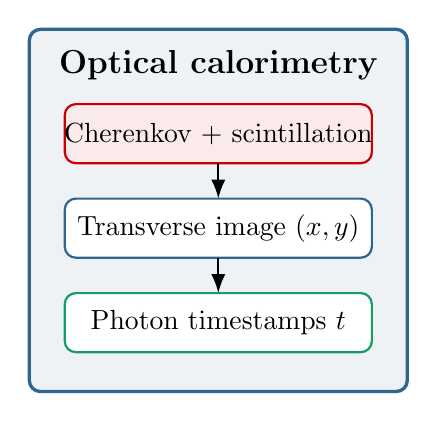
\begin{tikzpicture}[x=1cm,y=1cm]
        \draw[fill=Mist,draw=FlashBlue,very thick,rounded corners] (0,0) rectangle (4.8,4.6);
        \node[align=center,font=\bfseries\large] at (2.4,4.15) {Optical calorimetry};
        \draw[fill=PaleRed,draw=TTURed,thick,rounded corners] (0.45,2.9) rectangle (4.35,3.65);
        \node[align=center] at (2.4,3.27) {Cherenkov + scintillation};
        \draw[fill=white,draw=FlashBlue,thick,rounded corners] (0.45,1.7) rectangle (4.35,2.45);
        \node[align=center] at (2.4,2.07) {Transverse image $(x,y)$};
        \draw[fill=white,draw=FlashGreen,thick,rounded corners] (0.45,0.5) rectangle (4.35,1.25);
        \node[align=center] at (2.4,0.87) {Photon timestamps $t$};
        \draw[-{Latex[length=2.4mm]},thick] (2.4,2.9) -- (2.4,2.45);
        \draw[-{Latex[length=2.4mm]},thick] (2.4,1.7) -- (2.4,1.25);
      \end{tikzpicture}
    \end{column}
  \end{columns}
  \source{Motivation adapted from C. Madrid, \emph{Fiber Calorimetry at a Higgs Factory}, SLAC HFCC Workshop, Dec. 2024.}
\end{frame}

% 3
\begin{frame}{FLASH changes the unit of calorimeter information}
  \small
  \begin{columns}[T,onlytextwidth]
    \begin{column}{0.47\textwidth}
      \begin{beamercolorbox}[rounded=true,sep=0.28cm]{block body}
        \centering\bfseries Conventional SiPM chain
      \end{beamercolorbox}
      \vspace{0.18cm}
      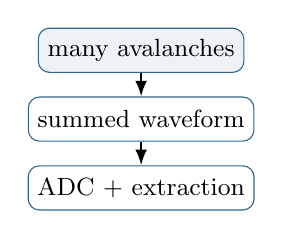
\begin{tikzpicture}[node distance=0.30cm,every node/.style={font=\small}]
        \node[draw=FlashBlue,rounded corners,fill=Mist,minimum width=2.45cm,minimum height=.56cm] (a) {many avalanches};
        \node[draw=FlashBlue,rounded corners,fill=white,below=of a,minimum width=2.45cm,minimum height=.56cm] (b) {summed waveform};
        \node[draw=FlashBlue,rounded corners,fill=white,below=of b,minimum width=2.45cm,minimum height=.56cm] (c) {ADC + extraction};
        \draw[-{Latex[length=2mm]},thick] (a)--(b);
        \draw[-{Latex[length=2mm]},thick] (b)--(c);
      \end{tikzpicture}
      \vspace{0.12cm}

      \footnotesize Integrated charge and a few waveform features. Dense sampling moves data continuously.
    \end{column}
    \begin{column}{0.05\textwidth}
      \centering\vspace{1.6cm}{\Large$\Longrightarrow$}
    \end{column}
    \begin{column}{0.47\textwidth}
      \begin{beamercolorbox}[rounded=true,sep=0.28cm]{block body}
        \centering\bfseries FLASH digital-SiPM chain
      \end{beamercolorbox}
      \vspace{0.18cm}
      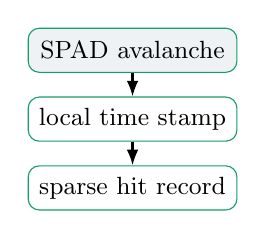
\begin{tikzpicture}[node distance=0.30cm,every node/.style={font=\small}]
        \node[draw=FlashGreen,rounded corners,fill=Mist,minimum width=2.65cm,minimum height=.56cm] (a) {SPAD avalanche};
        \node[draw=FlashGreen,rounded corners,fill=white,below=of a,minimum width=2.65cm,minimum height=.56cm] (b) {local time stamp};
        \node[draw=FlashGreen,rounded corners,fill=white,below=of b,minimum width=2.65cm,minimum height=.56cm] (c) {sparse hit record};
        \draw[-{Latex[length=2mm]},thick] (a)--(b);
        \draw[-{Latex[length=2mm]},thick] (b)--(c);
      \end{tikzpicture}
      \vspace{0.12cm}

      \footnotesize Export photon-level records only when light arrives, targeting $\mathcal{O}(10$--$50)$ ps timing.
    \end{column}
  \end{columns}
  \vspace{0.10cm}
  \begin{beamercolorbox}[rounded=true,sep=0.12cm]{alerted text}
    \centering\small\bfseries Physical SPAD pitch, timing-group size, and exported record granularity are three different design choices.
  \end{beamercolorbox}
  \source{FLASH public abstract, CALOR 2026: \href{https://indico.cern.ch/event/1572594/contributions/7106759/}{indico.cern.ch/event/1572594/contributions/7106759}.}
\end{frame}

% 4
\begin{frame}{Digital-SiPM architectures differ}
  \centering
  \fontsize{7.0}{8.0}\selectfont
  \renewcommand{\arraystretch}{1.08}
  \begin{tabularx}{\textwidth}{>{\bfseries}l >{\raggedright\arraybackslash}p{2.2cm} c c >{\raggedright\arraybackslash}X}
    \toprule
    Effort & Architecture & Pitch & Public timing & Maturity / caution \\
    \midrule
    FLASH & 3D SPAD + ASIC concept & scan: 5--100 $\mu$m & 10--50 ps target & Architecture is open; pitch must be quoted with PDE and recovery. \\
    Litavis & commercial dSiPM array & 10.17 $\mu$m & 37 ps TDC; 1145 ps IRF at 450 nm & Shows why TDC bin and photon-response timing must be separated. \\
    ASPIDES & monolithic HEP dSiPM & 30 $\mu$m & 100 ps TDC LSB & Submitted design; first/last timing plus counts. \\
    DESY & grouped SPAD prototype & $\sim$35 $\mu$m effective & $<100$ ps TDC; 50 ps MIP & Measured prototype; timing is shared within a larger pixel. \\
    DIGILOG & hybrid micro-SiPM + digital timing & 50 $\mu$m & 25 ps SPTR on test structures & Fast timing with analog grouping. \\
    Sherbrooke PDC & 3D-integrated platform & 78 $\mu$m & 130 ps SPAD FWHM & Measured sensor/ROIC platform; count/flag-oriented output. \\
    \bottomrule
  \end{tabularx}
\end{frame}

% 5
\begin{frame}{Published timing numbers answer different questions}
  \centering
  \includegraphics[height=0.67\textheight,width=0.96\textwidth,keepaspectratio]{assets/timing_landscape.png}
\end{frame}

% 6
\begin{frame}{Why benchmark FLASH with HG-DREAM?}
  \small
  \begin{columns}[T,onlytextwidth]
    \begin{column}{0.54\textwidth}
      \includegraphics[height=0.55\textheight,width=\linewidth,keepaspectratio]{assets/hgdream_high_granularity_crop.png}
    \end{column}
    \begin{column}{0.43\textwidth}
      \begin{itemize}\tightitem
        \item \key{Real optical shower density}: the core tests saturation and recovery, not only single-photon timing.
        \item \key{Two light components}: Cherenkov and scintillation probe different photon statistics and time structures.
        \item \key{Measured reference}: 2025 H8 data provide electrons, pions, muons, and protons for model closure.
        \item \key{Existing readout}: energy and fast-waveform paths let us compare sparse digital hits to current SiPM signals.
      \end{itemize}
    \end{column}
  \end{columns}
  \source{Y. Feng, \emph{Energy Performance of HG-DREAM with Test Beam}, CALOR 2026, slide 4.}
\end{frame}

% 7
\begin{frame}{HG-DREAM is now a measured system}
  \small
  \begin{columns}[T,onlytextwidth]
    \begin{column}{0.47\textwidth}
      \includegraphics[height=0.43\textheight,width=\linewidth,keepaspectratio,trim=0 70 0 0,clip]{assets/hgdream_fiber_layout.png}
      \vspace{0.12cm}
      \begin{beamercolorbox}[rounded=true,sep=0.18cm]{block body}
        \centering\small 4 Cherenkov + 3 scintillating fibers per 4 mm copper rod
      \end{beamercolorbox}
    \end{column}
    \begin{column}{0.50\textwidth}
      \vspace{0.05cm}
      \begin{tabular}{ccc}
        {\fontsize{22}{24}\selectfont\bfseries\color{TTURed}448} &
        {\fontsize{22}{24}\selectfont\bfseries\color{FlashBlue}896} &
        {\fontsize{22}{24}\selectfont\bfseries\color{FlashGreen}2 m} \\
        \scriptsize towers & \scriptsize channels & \scriptsize depth
      \end{tabular}
      \vspace{0.20cm}
      \begin{itemize}\tightitem
        \item 34 cm $\times$ 32 cm transverse size; 3 mm and 6 mm SiPMs.
        \item CAEN FERS energy readout plus 5 GHz, 12-bit DRS timing waveforms.
        \item 2025 H8 campaign studied calibration, leakage, dead/pathological channels, temperature, attenuation, noise, and GEANT4 agreement.
        \item Preliminary scintillation calibration gives about \key{60 photoelectrons/GeV}; Cherenkov yield is still being established.
      \end{itemize}
    \end{column}
  \end{columns}
  \source{Y. Feng, CALOR 2026, slides 7--8 and 24; \href{https://indico.cern.ch/event/1572594/contributions/7072387/}{public contribution page}.}
\end{frame}

% 8
\begin{frame}{Photon time carries shower-depth information}
  \small
  \begin{columns}[T,onlytextwidth]
    \begin{column}{0.58\textwidth}
      \vspace{0.05cm}
      \includegraphics[height=0.35\textheight,width=\linewidth,keepaspectratio]{assets/hgdream_timing_diagram.png}
    \end{column}
    \begin{column}{0.39\textwidth}
      \vspace{0.15cm}
      \[
        t_{\rm arrival}\simeq \frac{L_1}{c}+\frac{nL_2}{c}
      \]
      \footnotesize
      \begin{itemize}\tightitem
        \item Optical propagation is roughly \key{1 cm per 50 ps} in the fiber.
        \item A timestamp constrains where along the 2 m module the photon was produced.
        \item The observable is not only event time: it is the time-resolved shower profile.
      \end{itemize}
    \end{column}
  \end{columns}
  \vspace{0.10cm}
  \begin{beamercolorbox}[rounded=true,sep=0.10cm]{block body}
    \centering\footnotesize\bfseries HG-DREAM turns the FLASH timing target into a reconstruction question: how much longitudinal information survives the sensor and readout?
  \end{beamercolorbox}
  \source{Y. Feng, CALOR 2026, slide 5; C. Madrid, SLAC HFCC Workshop 2024, slide 12.}
\end{frame}

% 9
\begin{frame}{The benchmark closes a full measurement-to-model loop}
  \centering
  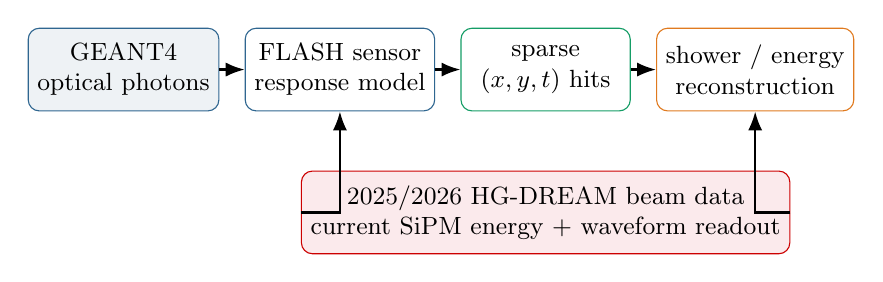
\begin{tikzpicture}[node distance=0.32cm,every node/.style={font=\small,align=center}]
    \node[draw=FlashBlue,fill=Mist,rounded corners,minimum width=2.15cm,minimum height=1.05cm] (g4) {GEANT4\\optical photons};
    \node[draw=FlashBlue,fill=white,rounded corners,right=of g4,minimum width=2.15cm,minimum height=1.05cm] (sensor) {FLASH sensor\\response model};
    \node[draw=FlashGreen,fill=white,rounded corners,right=of sensor,minimum width=2.15cm,minimum height=1.05cm] (hits) {sparse\\$(x,y,t)$ hits};
    \node[draw=FlashOrange,fill=white,rounded corners,right=of hits,minimum width=2.15cm,minimum height=1.05cm] (reco) {shower / energy\\reconstruction};
    \draw[-{Latex[length=2.4mm]},thick] (g4)--(sensor);
    \draw[-{Latex[length=2.4mm]},thick] (sensor)--(hits);
    \draw[-{Latex[length=2.4mm]},thick] (hits)--(reco);
    \node[draw=TTURed,fill=PaleRed,rounded corners,below=0.75cm of hits,minimum width=4.7cm,minimum height=1.05cm] (data) {2025/2026 HG-DREAM beam data\\current SiPM energy + waveform readout};
    \draw[-{Latex[length=2.4mm]},thick] (data.west) -| (sensor.south);
    \draw[-{Latex[length=2.4mm]},thick] (data.east) -| (reco.south);
  \end{tikzpicture}
  \vspace{0.45cm}
  \begin{columns}[T,onlytextwidth]
    \begin{column}{0.48\textwidth}
      \begin{beamercolorbox}[rounded=true,sep=0.25cm]{block body}
        \centering\bfseries Near term\par
        \small Constrain pitch, recovery, PDE, timing response, grouping, and output volume on existing samples.
      \end{beamercolorbox}
    \end{column}
    \begin{column}{0.48\textwidth}
      \begin{beamercolorbox}[rounded=true,sep=0.25cm]{block body}
        \centering\bfseries Prototype era\par
        \small Replace assumptions with measured FLASH parameters and validate the sparse representation against beam data.
      \end{beamercolorbox}
    \end{column}
  \end{columns}
\end{frame}

% 10
\begin{frame}{First audit the photon samples}
  \begin{columns}[T,onlytextwidth]
    \begin{column}{0.60\textwidth}
      \includegraphics[height=0.53\textheight,width=\linewidth,keepaspectratio]{assets/photon_xy_comparison.png}
    \end{column}
    \begin{column}{0.37\textwidth}
      \small
      \begin{itemize}\tightitem
        \item 5,000 events in each sample.
        \item One Cherenkov production fiber; 0--40 ns gate.
        \item Median photons/event: \key{127} for 100 GeV $e^+$ and \key{289} for 1 TeV $\pi^+$.
        \item Pion 90th percentile: \key{920}; maximum: \key{2,108}.
        \item Selected coordinates span about 0.8 mm: the physical fiber face.
      \end{itemize}
    \end{column}
  \end{columns}
  \vspace{0.05cm}
  \begin{beamercolorbox}[rounded=true,sep=0.12cm]{alerted text}
    \centering\footnotesize The energies are different. These are two occupancy stress samples, not a controlled particle-species comparison.
  \end{beamercolorbox}
  \source{DREAMSim 100 GeV positron and 1 TeV pion samples; this work.}
\end{frame}

% 11
\begin{frame}{The historical result reproduces exactly---as software closure}
  \begin{columns}[T,onlytextwidth]
    \begin{column}{0.56\textwidth}
      \includegraphics[height=0.53\textheight,width=\linewidth,keepaspectratio]{assets/validation_historical_closure.png}
    \end{column}
    \begin{column}{0.41\textwidth}
      \small
      \begin{itemize}\tightitem
        \item ROOT object names, binning, and integrals match the saved electron reference.
        \item Independent one-hit/event and 40 ns recovery implementations agree point by point.
        \item This validates the recovered algorithm and provenance.
      \end{itemize}
      \vspace{0.22cm}
      \begin{beamercolorbox}[rounded=true,sep=0.20cm]{alerted text}
        \centering\bfseries Closure does not prove that the coordinate convention represented physical pitch.
      \end{beamercolorbox}
    \end{column}
  \end{columns}
\end{frame}

% 12
\begin{frame}{Audit finding: the old pitch was three times too fine}
  \centering
  \includegraphics[height=0.54\textheight,width=0.97\textwidth,keepaspectratio]{assets/v2_mapping_correction.png}
  \vspace{0.02cm}
  \begin{beamercolorbox}[rounded=true,sep=0.12cm,wd=0.94\textwidth]{alerted text}
    \centering\footnotesize The old code divided a 3 mm sensor width into pitch-sized bins, then applied those bins to a 1 mm fiber-local display coordinate. A labelled 25 $\mu$m point therefore behaved like roughly 8.3 $\mu$m in physical DREAMSim coordinates.
  \end{beamercolorbox}
\end{frame}

% 13
\begin{frame}{The physical requirement is a surface, not one pitch}
  \centering
  \includegraphics[height=0.57\textheight,width=0.98\textwidth,keepaspectratio]{assets/v2_physical_requirements.png}
  \vspace{-0.03cm}
  \begin{beamercolorbox}[rounded=true,sep=0.11cm,wd=0.94\textwidth]{block body}
    \centering\footnotesize For the 1 TeV pion stress sample, survival depends jointly on pitch, PDE, and recovery. Lower PDE relieves collisions but also removes photons, so usable yield and recovery survival must both be reported.
  \end{beamercolorbox}
\end{frame}

% 14
\begin{frame}{Bright-event tails set a stronger requirement}
  \centering
  \includegraphics[height=0.57\textheight,width=0.92\textwidth,keepaspectratio]{assets/v2_event_tail.png}
  \vspace{-0.02cm}
  \begin{beamercolorbox}[rounded=true,sep=0.11cm,wd=0.90\textwidth]{alerted text}
    \centering\footnotesize At 20\% PDE and 4.3 ns recovery, the 10th-percentile event retains 96.7\%, 90.3\%, and 86.2\% at 10, 20, and 25 $\mu$m. A sample-average curve hides this risk.
  \end{beamercolorbox}
\end{frame}

% 15
\begin{frame}{Recovery distorts the pulse, not only the count}
  \centering
  \includegraphics[height=0.57\textheight,width=0.93\textwidth,keepaspectratio]{assets/v2_pulse_shape.png}
  \vspace{-0.04cm}
  \begin{beamercolorbox}[rounded=true,sep=0.10cm,wd=0.92\textwidth]{block body}
    \centering\footnotesize Collisions concentrate near the prompt peak. Coarser pitch preferentially suppresses early photons and can bias any timing-derived shower observable.
  \end{beamercolorbox}
\end{frame}

% 16
\begin{frame}{A first physics proxy changes the timing question}
  \centering
  \includegraphics[height=0.54\textheight,width=0.88\textwidth,keepaspectratio]{assets/v2_timing_depth.png}
  \vspace{-0.02cm}
  \begin{beamercolorbox}[rounded=true,sep=0.11cm,wd=0.92\textwidth]{alerted text}
    \centering\footnotesize The 10\% arrival-time quantile predicts mean photon-production depth with a tail-sensitive 236 mm RMSE. Adding 10--50 ps response/TDC smearing changes that RMSE by less than 0.1 mm; the simple observable, optical tails, and readout policy dominate first.
  \end{beamercolorbox}
\end{frame}

% 17
\begin{frame}{What the present samples support}
  \centering
  \small
  \renewcommand{\arraystretch}{1.28}
  \begin{tabular}{rccc}
    \toprule
    Physical pitch & Usable / incident & Recovery survival & 10th-percentile event survival \\
    \midrule
    10 $\mu$m & 19.64\% & 97.93\% & 96.7\% \\
    \rowcolor{Mist}20 $\mu$m & 18.59\% & 92.73\% & 90.3\% \\
    25 $\mu$m & 17.95\% & 89.50\% & 86.2\% \\
    \bottomrule
  \end{tabular}
  \vspace{0.30cm}
  \begin{columns}[T,onlytextwidth]
    \begin{column}{0.48\textwidth}
      \begin{beamercolorbox}[rounded=true,sep=0.20cm]{block body}
        \centering\bfseries Supported now\par
        \footnotesize A 10--20 $\mu$m physical-pitch region is worth prototyping under the 20\% PDE, 4.3 ns assumption.
      \end{beamercolorbox}
    \end{column}
    \begin{column}{0.48\textwidth}
      \begin{beamercolorbox}[rounded=true,sep=0.20cm]{alerted text}
        \centering\bfseries Not supported yet\par
        \footnotesize A universal pitch requirement, a calorimeter resolution claim, or a 10 ps system requirement.
      \end{beamercolorbox}
    \end{column}
  \end{columns}
  \source{1 TeV pion stress sample; 20\% constant PDE; 4.3 ns non-paralyzable recovery.}
\end{frame}

% 18
\begin{frame}{The next studies must close the physics loop}
  \scriptsize
  \renewcommand{\arraystretch}{1.18}
  \begin{tabularx}{\textwidth}{c >{\bfseries}p{3.1cm} X >{\raggedright\arraybackslash}p{2.2cm}}
    \toprule
    Priority & Study & Decision it enables & Deliverable \\
    \midrule
    1 & Matched-energy samples & Separate energy, particle type, and shower density. & $e/\pi/\mu$ at 10--300 GeV \\
    2 & Measured optical response & Replace constant PDE and Gaussian timing with FLASH/SiPM data. & PDE$(\lambda)$, IRF, recovery \\
    3 & Output-policy information & Compare all hits, first/last, grouped TDCs, and short histograms. & Depth/PID versus bits/event \\
    4 & Full-tile + beam closure & Move beyond one fiber and validate waveforms before sparse digitization. & Simulation--beam residuals \\
    \bottomrule
  \end{tabularx}
  \vspace{0.20cm}
  \begin{beamercolorbox}[rounded=true,sep=0.16cm]{alerted text}
    \centering\bfseries Immediate simulation campaign: matched-energy production plus output-policy baselines, before returning to neural networks.
  \end{beamercolorbox}
\end{frame}

% 19
\begin{frame}{LDRD loop: simulation knobs become measurements}
  \begin{columns}[T,onlytextwidth]
    \begin{column}{0.46\textwidth}
      \begin{beamercolorbox}[rounded=true,sep=0.24cm]{block body}
        \centering\bfseries Prototype measurements
      \end{beamercolorbox}
      \begin{itemize}\tightitem
        \item PDE versus wavelength and overvoltage
        \item recovery / hold-off distribution
        \item SPTR and time walk versus wavelength
        \item dark counts, crosstalk, afterpulsing
        \item hot-cell masking and operating temperature
      \end{itemize}
    \end{column}
    \begin{column}{0.06\textwidth}
      \centering\vspace{1.6cm}{\Large$\Longleftrightarrow$}
    \end{column}
    \begin{column}{0.46\textwidth}
      \begin{beamercolorbox}[rounded=true,sep=0.24cm]{block body}
        \centering\bfseries HG-DREAM validation
      \end{beamercolorbox}
      \begin{itemize}\tightitem
        \item photon yield and occupancy by fiber type
        \item waveform-to-hit representation tests
        \item longitudinal timing reconstruction
        \item dual-readout energy and PID observables
        \item output volume, buffering, and power envelope
      \end{itemize}
    \end{column}
  \end{columns}
  \vspace{0.16cm}
  \begin{beamercolorbox}[rounded=true,sep=0.18cm]{alerted text}
    \centering\normalsize\bfseries The benchmark is useful because it couples sensor specifications to a physics observable and an existing beam-test data set.
  \end{beamercolorbox}
\end{frame}

% 20
\begin{frame}{Takeaways}
  \small
  \vspace{0.03cm}
  \begin{enumerate}\tightitem
    \item \key{FLASH has a physics benchmark}: HG-DREAM connects sparse photon hits to dense optical showers, 2 m timing leverage, and beam data.
    \item \key{The audit changed the numerical conclusion}: the historical 3:1 coordinate convention made labelled pitches act three times finer than physical pitch.
    \item \key{There is no universal 25 $\mu$m point}: physical pitch must be specified with PDE, recovery, event tails, and output policy.
    \item \key{The next decisive result is information versus bandwidth}: matched samples and measured sensor response should connect sparse hits to shower-depth and dual-readout performance.
  \end{enumerate}
  \vspace{0.18cm}
  \begin{beamercolorbox}[rounded=true,sep=0.13cm]{block body}
    \centering\fontsize{12.5}{15}\selectfont\bfseries
    The CPAD message: FLASH is a sensor-development program tied to a real calorimeter, real photon densities, and a measurable reconstruction payoff.
  \end{beamercolorbox}
\end{frame}

\appendix

% B1
\begin{frame}{Backup: input audit and cutflow}
  \small
  \renewcommand{\arraystretch}{1.16}
  \begin{tabular}{lrr}
    \toprule
    Sequential selection & 100 GeV $e^+$ & 1 TeV $\pi^+$ \\
    \midrule
    Raw optical photons & 2,629,165 & 7,722,345 \\
    Core Cherenkov, downstream exit & 2,629,165 & 7,722,345 \\
    Inside 0--40 ns & 2,624,844 & 7,708,802 \\
    Production fiber 0 & 649,310 & 1,899,950 \\
    Inside centered 3 mm sensor & 649,310 & 1,899,950 \\
    \bottomrule
  \end{tabular}
  \vspace{0.30cm}
  \begin{beamercolorbox}[rounded=true,sep=0.18cm]{block body}
    \centering\footnotesize No selected fiber-0 photon is lost at the physical 3 mm sensor boundary. The photon cloud spans only about $-0.39$ to $+0.40$ mm in each coordinate.
  \end{beamercolorbox}
  \source{Machine-readable cutflow in \texttt{results/flash-study-v2-final/input\_selection\_audit.json}.}
\end{frame}

% B2
\begin{frame}{Backup: old and new code close exactly}
  \centering
  \includegraphics[height=0.50\textheight,width=0.96\textwidth,keepaspectratio]{assets/validation_historical_closure.png}
  \vspace{0.02cm}
  \begin{beamercolorbox}[rounded=true,sep=0.12cm,wd=0.88\textwidth]{alerted text}
    \centering\footnotesize At every shared pitch, the independent 40 ns recovery calculation reproduces the historical one-hit-per-event efficiency with zero numerical difference.
  \end{beamercolorbox}
  \source{Historical reproduction output and full-sample pitch/recovery scan; this work.}
\end{frame}

% B3
\begin{frame}{Backup: how the factor-of-three entered}
  \small
  \begin{tabularx}{\textwidth}{>{\bfseries}p{3.3cm} X}
    \toprule
    Quantity & Historical implementation \\
    \midrule
    Segmentation & $N_{\rm bins}=3000\,\mu\mathrm{m}/p_{\rm labelled}$ \\
    Coordinate range & fiber-local plot range $[-0.5,+0.5)$ mm \\
    Implemented cell width & $1\,\mathrm{mm}/N_{\rm bins}=p_{\rm labelled}/3$ \\
    Example & 25 $\mu$m label $\rightarrow$ 120 bins $\rightarrow$ 8.3 $\mu$m physical cell \\
    Corrected mapping & physical millimeters retained; centered sensor $[-1.5,+1.5)$ mm \\
    Historical products & retained unchanged as exact software/provenance closure \\
    \bottomrule
  \end{tabularx}
\end{frame}

% B4
\begin{frame}{Backup: corrected physical working-region values}
  \centering
  \small
  \renewcommand{\arraystretch}{1.25}
  \begin{tabular}{rccc}
    \toprule
    Pitch & Usable / incident & Accepted / detected & 10th-percentile event \\
    \midrule
    10 $\mu$m & 19.64\% & 97.93\% & 96.7\% \\
    20 $\mu$m & 18.59\% & 92.73\% & 90.3\% \\
    25 $\mu$m & 17.95\% & 89.50\% & 86.2\% \\
    \bottomrule
  \end{tabular}
  \vspace{0.45cm}

  \begin{beamercolorbox}[rounded=true,sep=0.24cm,wd=0.83\textwidth]{block body}
    \centering 1 TeV pion stress sample; 20\% constant PDE; 4.3 ns recovery. The first column includes PDE loss; the second isolates recovery loss.
  \end{beamercolorbox}
\end{frame}

% B5
\begin{frame}{Backup: public benchmark sources}
  \fontsize{8.5}{10}\selectfont
  \begin{itemize}\tightitem
    \item FLASH abstract: \url{https://indico.cern.ch/event/1572594/contributions/7106759/}
    \item HG-DREAM status: \url{https://indico.cern.ch/event/1572594/contributions/7072387/}
    \item Litavis datasheet: \url{https://singularphotonics.com/wp-content/uploads/2026/09/SP-Litavis-Datasheet-0926.pdf}
    \item ASPIDES: \url{https://indico.cern.ch/event/1608852/contributions/6815865/}
    \item DESY prototype: \url{https://arxiv.org/abs/2402.12305}
    \item DIGILOG: \url{https://indico.cern.ch/event/1473071/contributions/6462208/}
    \item Philips DPC3200: \url{https://cds.cern.ch/record/2255746/}
    \item Sherbrooke PDC platform: \url{https://imagesensors.org/Past\%20Workshops/2024\%20ISSW/Posters/P2-09.pdf}
  \end{itemize}
  \vspace{0.25cm}
  \small Every plotted number is stored with its timing definition, maturity, pitch basis, and source in \texttt{cpad\_benchmarks.json}.
\end{frame}

% B6
\begin{frame}{Backup: what is not in the present requirement yet}
  \begin{columns}[T,onlytextwidth]
    \begin{column}{0.47\textwidth}
      \begin{beamercolorbox}[rounded=true,sep=0.22cm]{block body}
        \centering\bfseries Sensor effects
      \end{beamercolorbox}
      \begin{itemize}\tightitem
        \item wavelength-dependent PDE
        \item fill factor and optical coupling
        \item dark counts and hot cells
        \item crosstalk and afterpulsing
        \item time walk and non-Gaussian timing tails
      \end{itemize}
    \end{column}
    \begin{column}{0.47\textwidth}
      \begin{beamercolorbox}[rounded=true,sep=0.22cm]{block body}
        \centering\bfseries System effects
      \end{beamercolorbox}
      \begin{itemize}\tightitem
        \item timing-group sharing
        \item TDC arbitration and buffer depth
        \item link bandwidth and event framing
        \item power and thermal constraints
        \item calibration and disabled-cell strategy
      \end{itemize}
    \end{column}
  \end{columns}
  \vspace{0.45cm}
  \begin{beamercolorbox}[rounded=true,sep=0.28cm]{alerted text}
    \centering\bfseries These omissions are why the present curves are design constraints, not final FLASH performance claims.
  \end{beamercolorbox}
\end{frame}

\end{document}
